\subsection{Subspaces and product spaces of fully lattice-ordered spaces}

Let E be a fully lattice-ordered space, H a linear subspace of E. The order structure induced on H by that of E is compatible with the vector space structure of H, but the ordered vector space H so defined is not necessarily a fully lattice-ordered space.

More precisely, it can happen that H is not a Riesz space (Exer. 2), or that H is a Riesz space but is not fully lattice-ordered: the latter is the case for the subspace \(\mathcal{C}(\mathbf{R})\) of the space \(\mathcal{B}(\mathbf{R})\) (No.~3, Example 2).

\pandocbounded{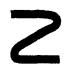
\includegraphics[keepaspectratio]{images/part001_ed0b989f.jpg}}

Moreover, if H is a Riesz space (fully lattice-ordered or not) it can happen that the supremum in H of two elements of H is different from their supremum in E (Exer. 3 b)). Finally, it can happen that H is fully lattice-ordered, that the supremum of each finite subset of H is the same in E and in H, but that there exist infinite subsets of H, bounded above in H, for which the suprema in E and H are different (Exer. 13 f)).

Let \((\mathrm{E}_{\iota})_{\iota \in \mathrm{I}}\) be any family of ordered vector spaces. Recall that, in the product space \(\mathrm{E} = \prod_{\iota \in \mathrm{I}}\mathrm{E}_{\iota}\) , the product order relation of the order relations of the factor spaces is the relation \(\ll x_{\iota}\leqslant y_{\iota}\) for all \(\iota \in \mathrm{I}\gg (\mathrm{S},\mathrm{III},\S 1,\mathrm{No.~4})\) . One verifies immediately that this relation is compatible with the vector space structure of E; E, equipped with this structure, is called the product space of the ordered spaces \(E_{\iota}\) .

PROPOSITION 3. --- Let \((\mathbf{E}_{\iota})_{\iota\in\mathbb{I}}\) be a family of ordered vector spaces. For the product space \(E=\prod_{\iota\in I}E_{\iota}\) to be a Riesz space (resp. a fully lattice-ordered space), it is necessary and sufficient that each of the spaces \(E_{\iota}\) be a Riesz space (resp. a fully lattice-ordered space).

Let us restrict ourselves to examining the case of fully lattice-ordered spaces. Suppose that all of the \(E_{\iota}\) are fully lattice-ordered; let A be a nonempty subset of E that is bounded above and let \(a = (a_{\iota})\) be an upper bound for A. For every \(\iota \in I\) , \(pr_{\iota}A\) is bounded above by \(a_{\iota}\) , hence has a supremum \(b_{\iota}\) in \(E_{\iota}\) ; it is clear that \(b = (b_{\iota})\) is the supremum of A in E.

Conversely, suppose E is fully lattice-ordered. Let \(A_{\kappa}\) be a subset of \(E_{\kappa}\) that is bounded above, \(A_{\kappa}^{\prime}\) the subset of E formed by the \(x = (x_{\iota})\) such that \(x_{\kappa} \in A_{\kappa}\) and \(x_{\iota} = 0\) for \(\iota \neq \kappa\) . It is immediate that \(A_{\kappa}^{\prime}\) is bounded above in E, hence has a supremum \(b = (b_{\iota})\) ; by the definition of the product order relation, necessarily \(b_{\iota} = 0\) for \(\iota \neq \kappa\) , and \(b_{\kappa}\) is the supremum of \(A_{\kappa}\) , which completes the proof.

DEFINITION 3. --- Let E be an ordered vector space, V and W two supplementary linear subspaces of E. One says that E is the ordered direct sum of V and W if the canonical mapping \((x,y)\mapsto x+y\) of the ordered vector space \(V\times W\) onto the ordered vector space E is an isomorphism.

PROPOSITION 4. --- For an ordered vector space E to be the ordered direct sum of two supplementary linear subspaces V, W, it is necessary and sufficient that the relations \(x \in V\) , \(y \in W\) , \(x + y \geqslant 0\) imply \(x \geqslant 0\) and \(y \geqslant 0\) .

Since \(x \geqslant 0\) and \(y \geqslant 0\) imply \(x + y \geqslant 0\) in E, the condition in the statement says that \((x, y) \mapsto x + y\) transforms the set of elements \(\geqslant 0\) of \(V \times W\) into the set of elements \(\geqslant 0\) of E.

